\documentclass[a4, UTF8]{article}
\usepackage{amsmath}
\usepackage{bm}
\usepackage{hyperref}
\usepackage{graphicx}
\begin{document}
\title{List of remarks and minor corrections\\
\large ``Interplay between Complex Orders in Functional Materials''\\
by\\
Dott Louis Ponet, Scuola Normale Superiore}
\date{}
\maketitle
{\bf Page 10:}~{\it The candidate states: ``Without loss of generality, we choose this point to be the gamma
point.'' This does not appear to be obvious, because not all T-invariant points are equivalent. Can
this be better explained?}
\\\\
% This is true. What is meant here is that for the purpose of the derivation only $\bm k_r = \bm k - \bm \bm k_0$ matters. Whether $\bm k_0 = \bm 0$ or another T-invariant point changes what the $|u_n, \sigma>$ are in Eq.(2.14).

{\bf Page 17:}~{\it Why is the exact experimental unit cell not used in this case? Is the unit cell used here the result of DFT optimisation?}
\\\\
No particular reason.
\\\\
{\bf Page 24, Fig.~2.9:}~{\it The direction of the path in reciprocal space is not clear on the axes.}
I have added $A \leftarrow Z \rightarrow U$ to this and the following figure.
\\\\
{\bf Page 36, Fig.~3.1:}~{\it This figure is not at all clear, partly due to the fact that only few spin directions are indicated. One should first of all sttate in the caption that the chains are AFM, but also indicate some of the spins so that the fragments in panels b) and c) can be identified in the larger structure.}
\\\\
Thank you for this suggestion, I have added the spins corresponding to ib) and c) in a).
I have also added a more explicit statement of the AFM nature of the chains in the caption.
\\\\
{\bf Page 37:}~{\it The candidate states that the electronic and lattice polarisations largely cancel in other members of the $R$Mn$_2$O$_5$ family but not in GdMn$_2$O$_5$. This is a bit of an exaggeration, as the polarisation in GdMn$_2$O$_5$ is not hugely different from YMn$_2$O$_5$, for example - perhaps restate.}
\\\\
This is a mistake, I misinterpreted some discussions on the comparison of ab-initio calculations on $R$Mn$_2$O$_5$, either neglecting or including on-site Coulomb repulsion, where it was shown that without including correlations the polarization is an order of magnitude larger (see e.g. \href{https://arxiv.org/abs/0802.0653v1}{Electronic correlations decimate the ferroelectric polarization of multiferroic HoMn$_2$O$_5$}). However this happens in ~{\it any} $R$Mn$_2$O$_5$, and so my wording was misleading at best. I have changed it to be more precise, refering to the above paper. 
\\\\
{\bf Page 38, Fig.~3.2:}~{\it It is really a pity that panel a) is inconsistent with previous measurements and with theory. Have these measurements been repeated?}
\\\\
Up to this point sadly not. We are also not entirely sure why this is happening, since the samples are identical as far as we know, and it is simply not possible to get the four-state behavior without having both two-state behaviors. We are currently working together with the experimentalists to further understand what is happening, and perform these low-angle measurements.
\\\\
{\bf Page 39, Fig.~3.3:}~{\it Some of the magnetic field scales are missing.}
\\\\
Fixed
\\\\
{\bf Page 44 and following:}~{\it The analysis provided in terms of individual spins is adequate but
inelegant. In general, this type of analysis is better done in terms of Fourier components with
terms properly related by symmetry via irrep transformations, leading to a set of order parameters.
For example, in the absence of a magnetic field, it is clear that Gd spins must transform with the
same irrep as Mn spins in order for coupling to exist. There may be a good reason why this is not
possible or convenient here – explain.}
\\\\
Initially we tried to indeed construct a model using this method, based on the description in the middle of page 3 of \href{https://link.aps.org/doi/10.1103/PhysRevLett.110.137203}{Giant Tunability of Ferroelectric Polarization in GdMn$_2$O$_5$}. This means we used the X$_2$ irrep and its modes to find the invariants. We found that this led to very complicated expressions and we made little progress through this way, after which we decided to try it in this more explicit way.
After finding that the model very well described the experiments, we tried to project the components of the spins and N\'eel vectors onto the X$_2$ modes during a field sweep. This is displayed in figure \ref{allirreps}.
\begin{figure}[h]
	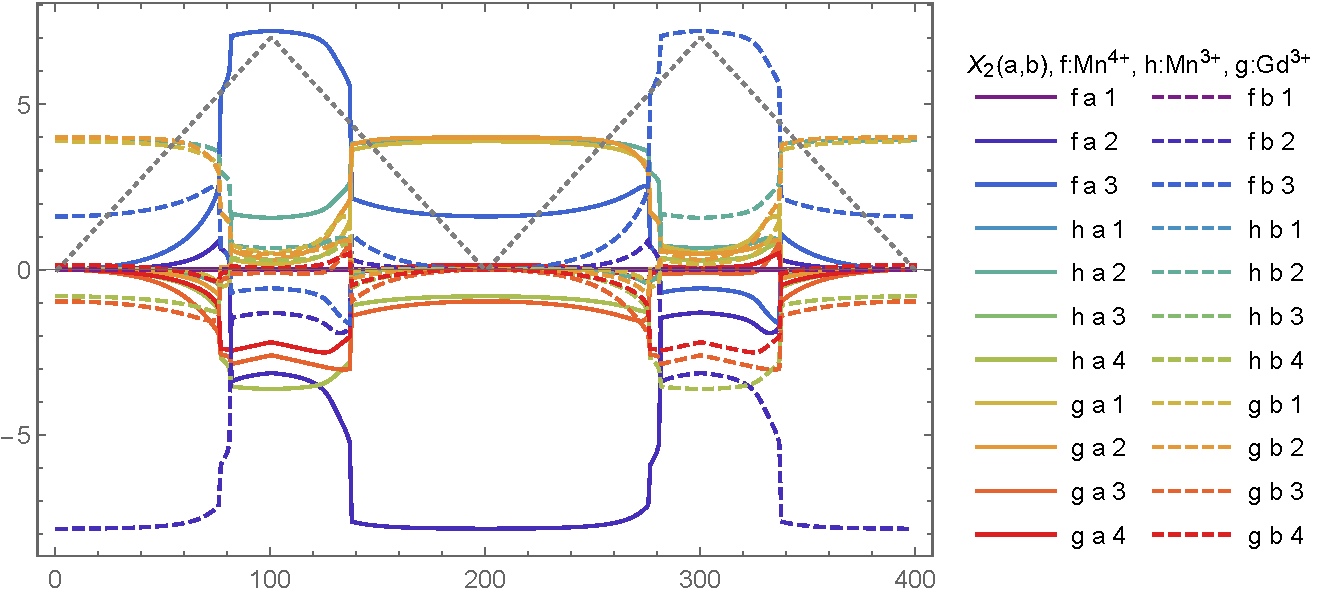
\includegraphics[width=\textwidth]{allIrreps.pdf}
	\caption{\label{allirreps}{\bf Projections onto X$_2$ modes.} The graphs represent the projections on the (a,b) components of the X$_2$ of the spins that are in the unit cell, during the double field sweep. The magnetic field amplitude is represented by the grey dotted graph. The three Wyckoff positions are labeled by $f$, $h$ and $g$ for the Mn$^{4+}$, Mn$^{3+}$, and Gd positions. The numbering denotes which spatially equivalent Wyckoff position the moment belongs to, and the full and dotted graphs denote the $a$ and $b$ components of each moment, respectively.}
\end{figure}
From the figure it is clear that the behavior of the projections of the spins is rather complex, and many require the full 2D projections to describe their evolution throughout the full cycle.
Our model is greatly simplified since, through the use of the unit vectors in the $ab$ plane, we have only one angle per spin as the variable.
\\\\
{\bf Page 50:}~{\it The candidate mentions the Nudged Elastic Band model which, however, is not introduced.}
\\\\
I have added a small description to the text:

The Nudged Elastic Band calculations are a way to track how the low points of the valley in Fig.~\ref{fig:GdMn2O5_heatmap} change for different field strengths.
This is done by taking two extremal states, then constructing a set of images that interpolate in phase space between these two states. The total energy of the entire chain is then optimized using a small elastic-like energy term that binds the images together, so that they find the lowest energy barrier between the two states.  
\\\\
{\bf Page 54, Fig.~3.10}~{\it I found this figure (especially the `squiggles' in panels b to f) extremely confusing. I am not sure it adds much, so I would consider omitting, but a better caption is certainly in order.}
\\\\
This figure was made in an attempt to summarize all the possible switching behaviors that can be found in the material. The squiggles are a way to demonstrate how the evolution of the AFM order parameter happens when the field is swept up and down, with the color gradient of panel (a) encoding the time evolution, which corresponds to the gradient of the squiggles.

I have changed the caption in an attempt to be more clear.
\\\\
{\bf Page 65, Fig.~4.1}~{\it }

\end{document}
